\section{The whole macromolecule}
\label{wholemacromolecule}

To regenerate the whole human \ttt{metHgb} macromolecule, we are going to follow basically the schema shown in \ffigure{fig:scipion_workflow_whole_reconstruction}. Starting from the symmetric unit, \chimera \ttt{operate} protocol allows to generate the whole molecule by symmetry. As in the previous step, validation programs drive to selection of the best $model$ of the whole molecule after one or several rounds of assessment - refinement -assessment. A final validation step will be accomplished with \chimera \ttt{map subtraction} protocol to assess the volume density occupancy of the new macromolecule generated.

\begin{itemize}

 \item Protocol \scommand{chimerax - operate} to generate the whole molecule of human \ttt{Hgb}:\\
 
 Following previous instructions, open \chimera \ttt{operate} protocol (\ffigure{fig:chimera_operate_protocol} (1)), load 
 the selected atomic structure $model$ of \ttt{metHgb} asymmetric unit (2), and execute the protocol (3). \chimera graphics interface will show you the $model$ of \ttt{metHgb} asymmetric unit. Considering the C2 symmetry of the whole molecule, write in \chimera command line to re-generate the whole molecule:\\
 
 \ttt{sym \#2 C2 copies true}\\
 
 A symmetric image of the input $model$ (\ffigure{fig:chimera_operate_sym}; $model$ \ttt{\#2}) will be generated. The new $model$ \ttt{\#3} contains both the input (\ffigure{fig:chimera_operate_sym}, \iii{model} \ttt{\#3.1})and the symmetric unit (\iii{model} \ttt{\#3.2}), and the whole structure can be saved by writing in \chimera command line:\\
 
 \ttt{scipionwrite \#3 prefix whole\_model\_}
 
 \begin{figure}[H]
    \centering 
    \captionsetup{width=.9\linewidth} 
    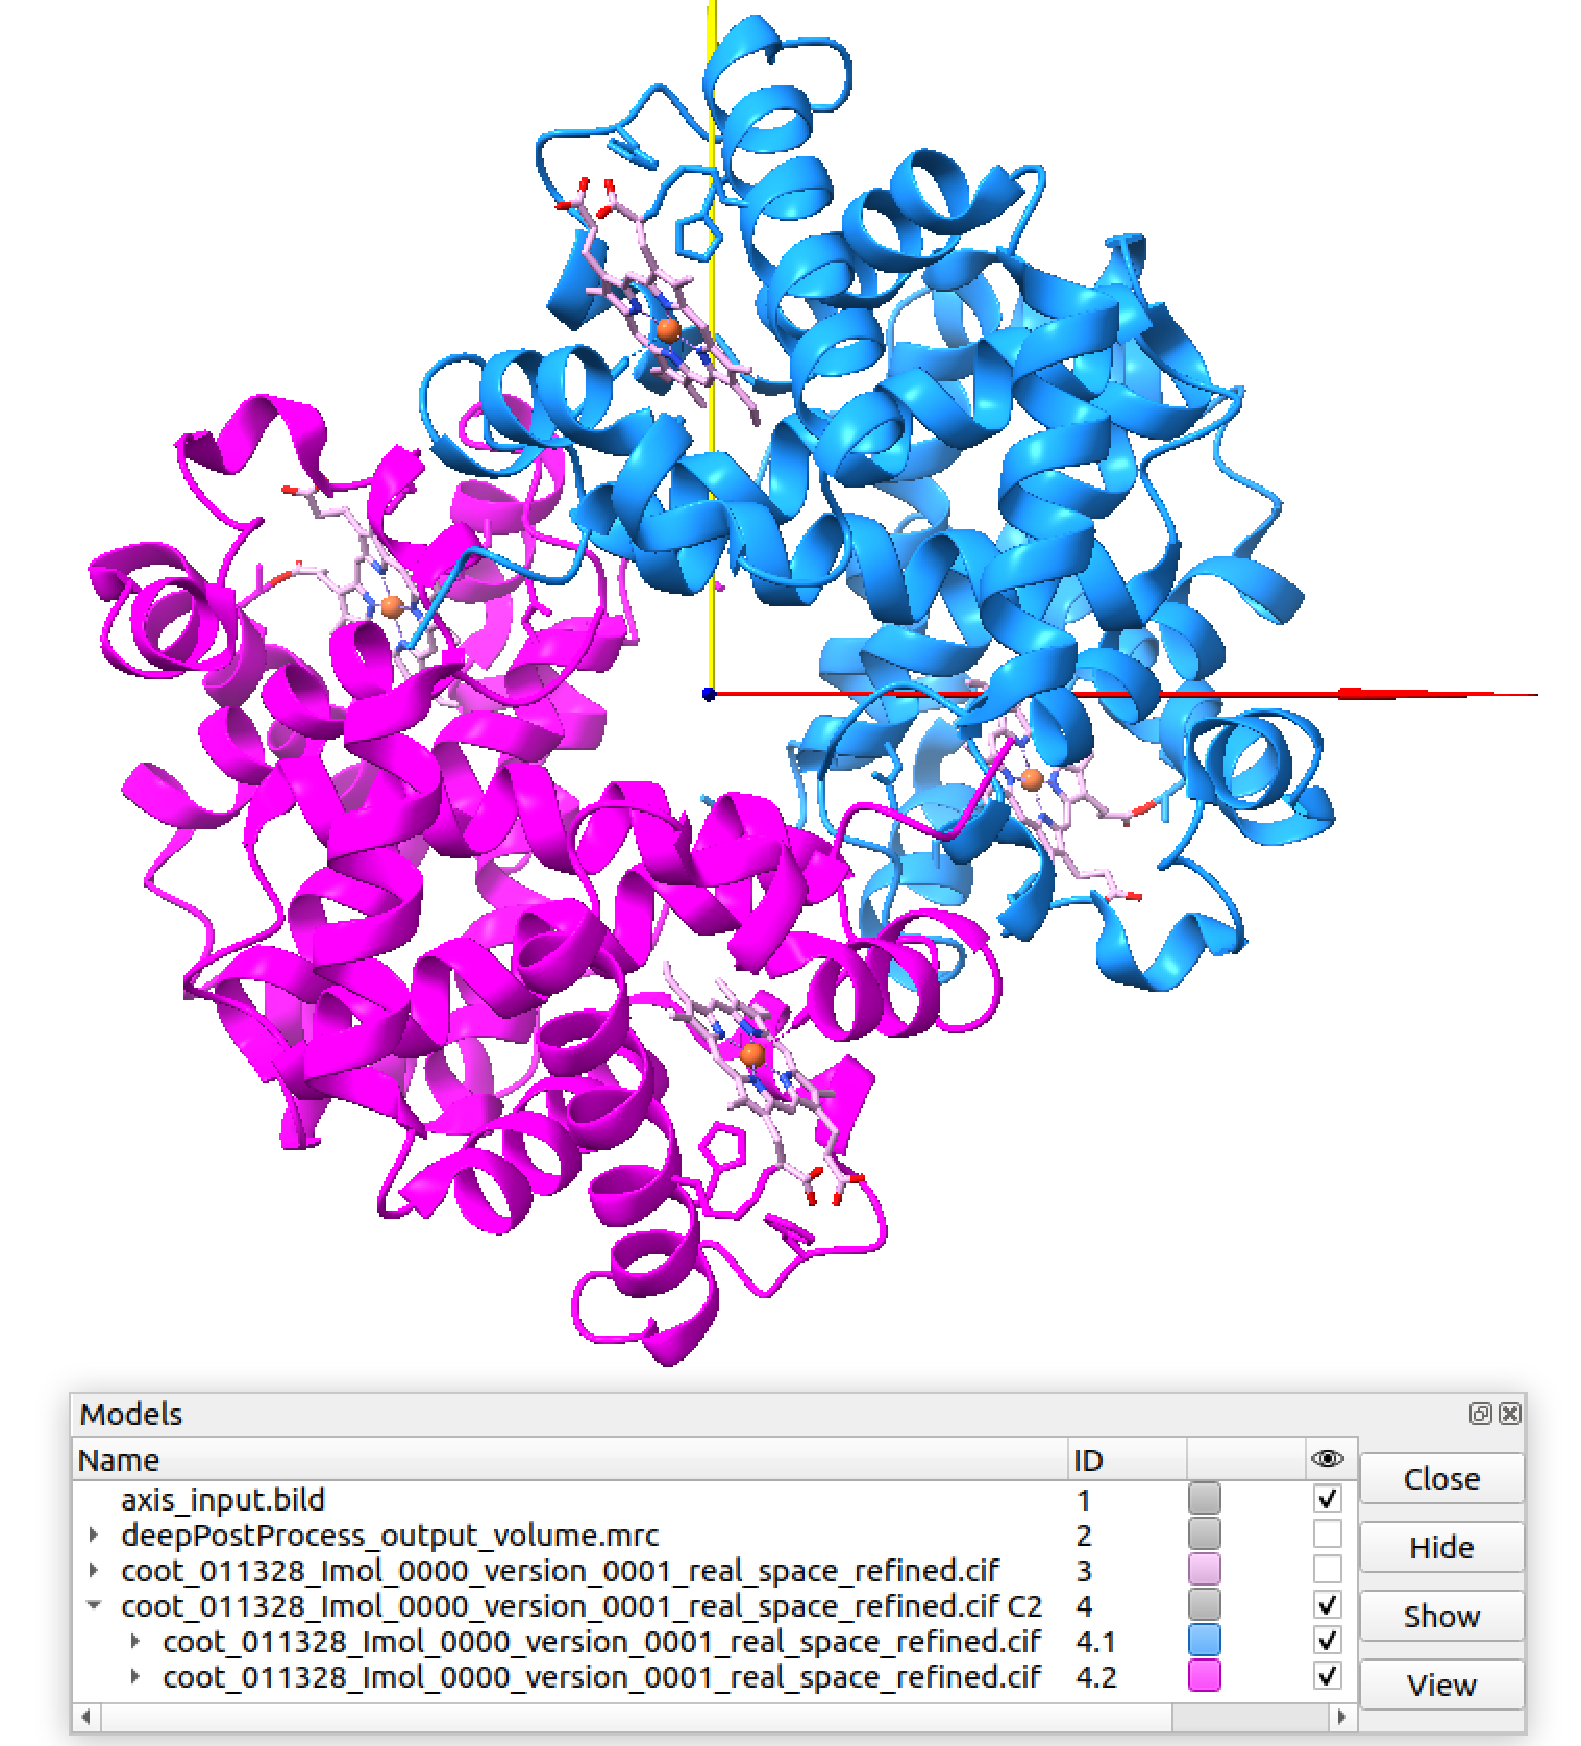
\includegraphics[width=0.50\textwidth]{Images/Fig41}
    \caption{$Model$ generated for the whole human \ttt{metHgb}.}
    \label{fig:chimera_operate_sym}
   \end{figure}
 
 \ttt{Note}: In this small example selected for modeling it doesn't matter if we model the map asymmetric unit or the whole molecule. However, in real life to model the whole molecule doesn't make sense because of its huge size. In that case, we will limit our modeling to the map asymmetric unit. The right modeling of this part of the molecule will require to add the adjacent asymmetric units in order to perform the appropriate modeling of the overlapping areas, avoiding steric classes in the reconstruction by symmetry of the whole molecule. In that case, the command lines would be:
    \begin{itemize}
     \item To generate the symmetry copies:\\
     \ttt{sym \#2 C2 copies true}\\
      \item To remove in the new \iii{model} \ttt{\#3} the symmetry copies with centers within a certain range of distance \ttt{d} of the center of the molecule input \iii{model}:\\
      \ttt{delete \#3 \& \#2 \#>d}
    \end{itemize}
At this point we will continue with the refinement process of this asymmetric unit plus neighbors. The validation will focus only in the asymmetric unit, which will be recovered by removing the remaining adjacent asymmetric units. This cleaning or removing of the neighbor units can be performed with the protocol \chimera \ttt{operate} each time we would like to validate the structure.
 
 
 \item Protocols to refine the new combined structure generated:\\
  
As we said in the previous chapter regarding the building of the asymmetric unit, refinements should cover specially the overlapping areas between the two asymmetric units. Help yourself with the \coot tools of \ttt{Validate} in the main menu, as well as the visualization tools of \phenix \ttt{real space refine} protocol. 
 \item Validation protocols to select the best $model$ of the whole human \ttt{Hgb}:\\
 
 \emringer and $Validation CryoEM (MolProbity)$ statistics have to be computed for the new $model$ of the whole human \ttt{metHgb} obtained by using \chimera \ttt{operate} protocol (see results \ttable{table:refmac_question_12} in Appendix \ref{app:solutions}; \textbf{Question \ref{wholemacromolecule}\_1}). Because of high values of \ccmask and \emringer \ttt{score}, as well as acceptable \molprobity statistics, $model$ generated by \chimera \ttt{operate} protocol is selected as $model$ of the whole human \ttt{metHgb}. Additional refinement steps with \phenix \ttt{real space refine} and \refmac do not seem to improve the result significantly. In this case, RMSD value of the selected atomic structure $model$, regarding the published structure, yields an intermediate value between the best and the worst one.\\
 
 \item Protocol \scommand{chimerax - map subtraction} to assess volume density occupancy:\\
 
 We perform this analysis in order to identify part of the density map that were not modeled previously, maybe unknown parts of the complex. Sometimes the density level or the resolution in these areas differ from the rest of the map and commonly are more blurry, which makes much more difficult to identify and trace them. Ideally, we would like to remove the map density associated to the already traced atomic structure to facilitate the modeling of the remnant density. Obviously, there are some limitations in this process. We will run a protocol based on \chimera (Appendix \ref{app:chimeraMapSubtraction}) to subtract the modeled part of the map from the whole map.
 
 As we have seen previously, open \chimera \ttt{operate} protocol (\ffigure{fig:chimera_operate_protocol} (1)), load both the initial volume and the selected atomic structure $model$ of the whole human \ttt{metHgb} (2), and execute the protocol (3). \ffigure{fig:chimera_operate_vol} shows the initial volume \ttt{EMD-3488} (grey) and the selected $model$ that we have traced for human \ttt{metHgb} (pink):
 
 \begin{figure}[H]
    \centering 
    \captionsetup{width=.7\linewidth} 
    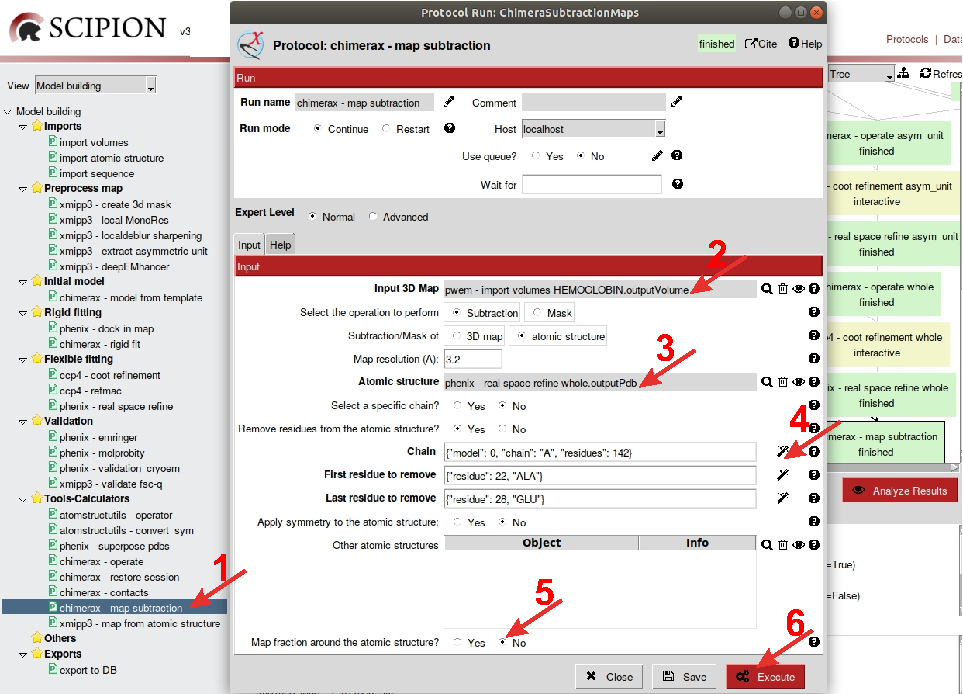
\includegraphics[width=0.90\textwidth]{Images/Fig42}
    \caption{Human \ttt{metHgb} $model$ opened by \chimera \ttt{operate} protocol.}
    \label{fig:chimera_operate_vol}
   \end{figure}
 
 To check if the selected model of \ttt{metHgb} occupies most part of the starting volume, we have to compare by subtraction the $model$-derived volume and the starting volume \ttt{EMD-3488}. To perform this operation, follow the next two steps:
 
  \begin{itemize}
  
  \item To generate a volume from the $model$ at 3.307\AA\ resolution (resolution shown in \phenix-\ttt{\molprobity viewer}; \ttt{Real space correlation}; \ttt{Atom Mask Radius}), write in \chimera command line:\\
  
  \ttt{molmap \#2 3.307 modelId 3}\\
  
  Next \ffigure{fig:chimera_operate_vol_2} shows the volume (\iii{Chimera model} \#3) generated in \chimera at 3.307\AA\ resolution, starting from the selected atomic structure of human \ttt{metHgb} (\iii{Chimera model} \#2). 
   
  \begin{figure}[H]
    \centering 
    \captionsetup{width=.7\linewidth} 
    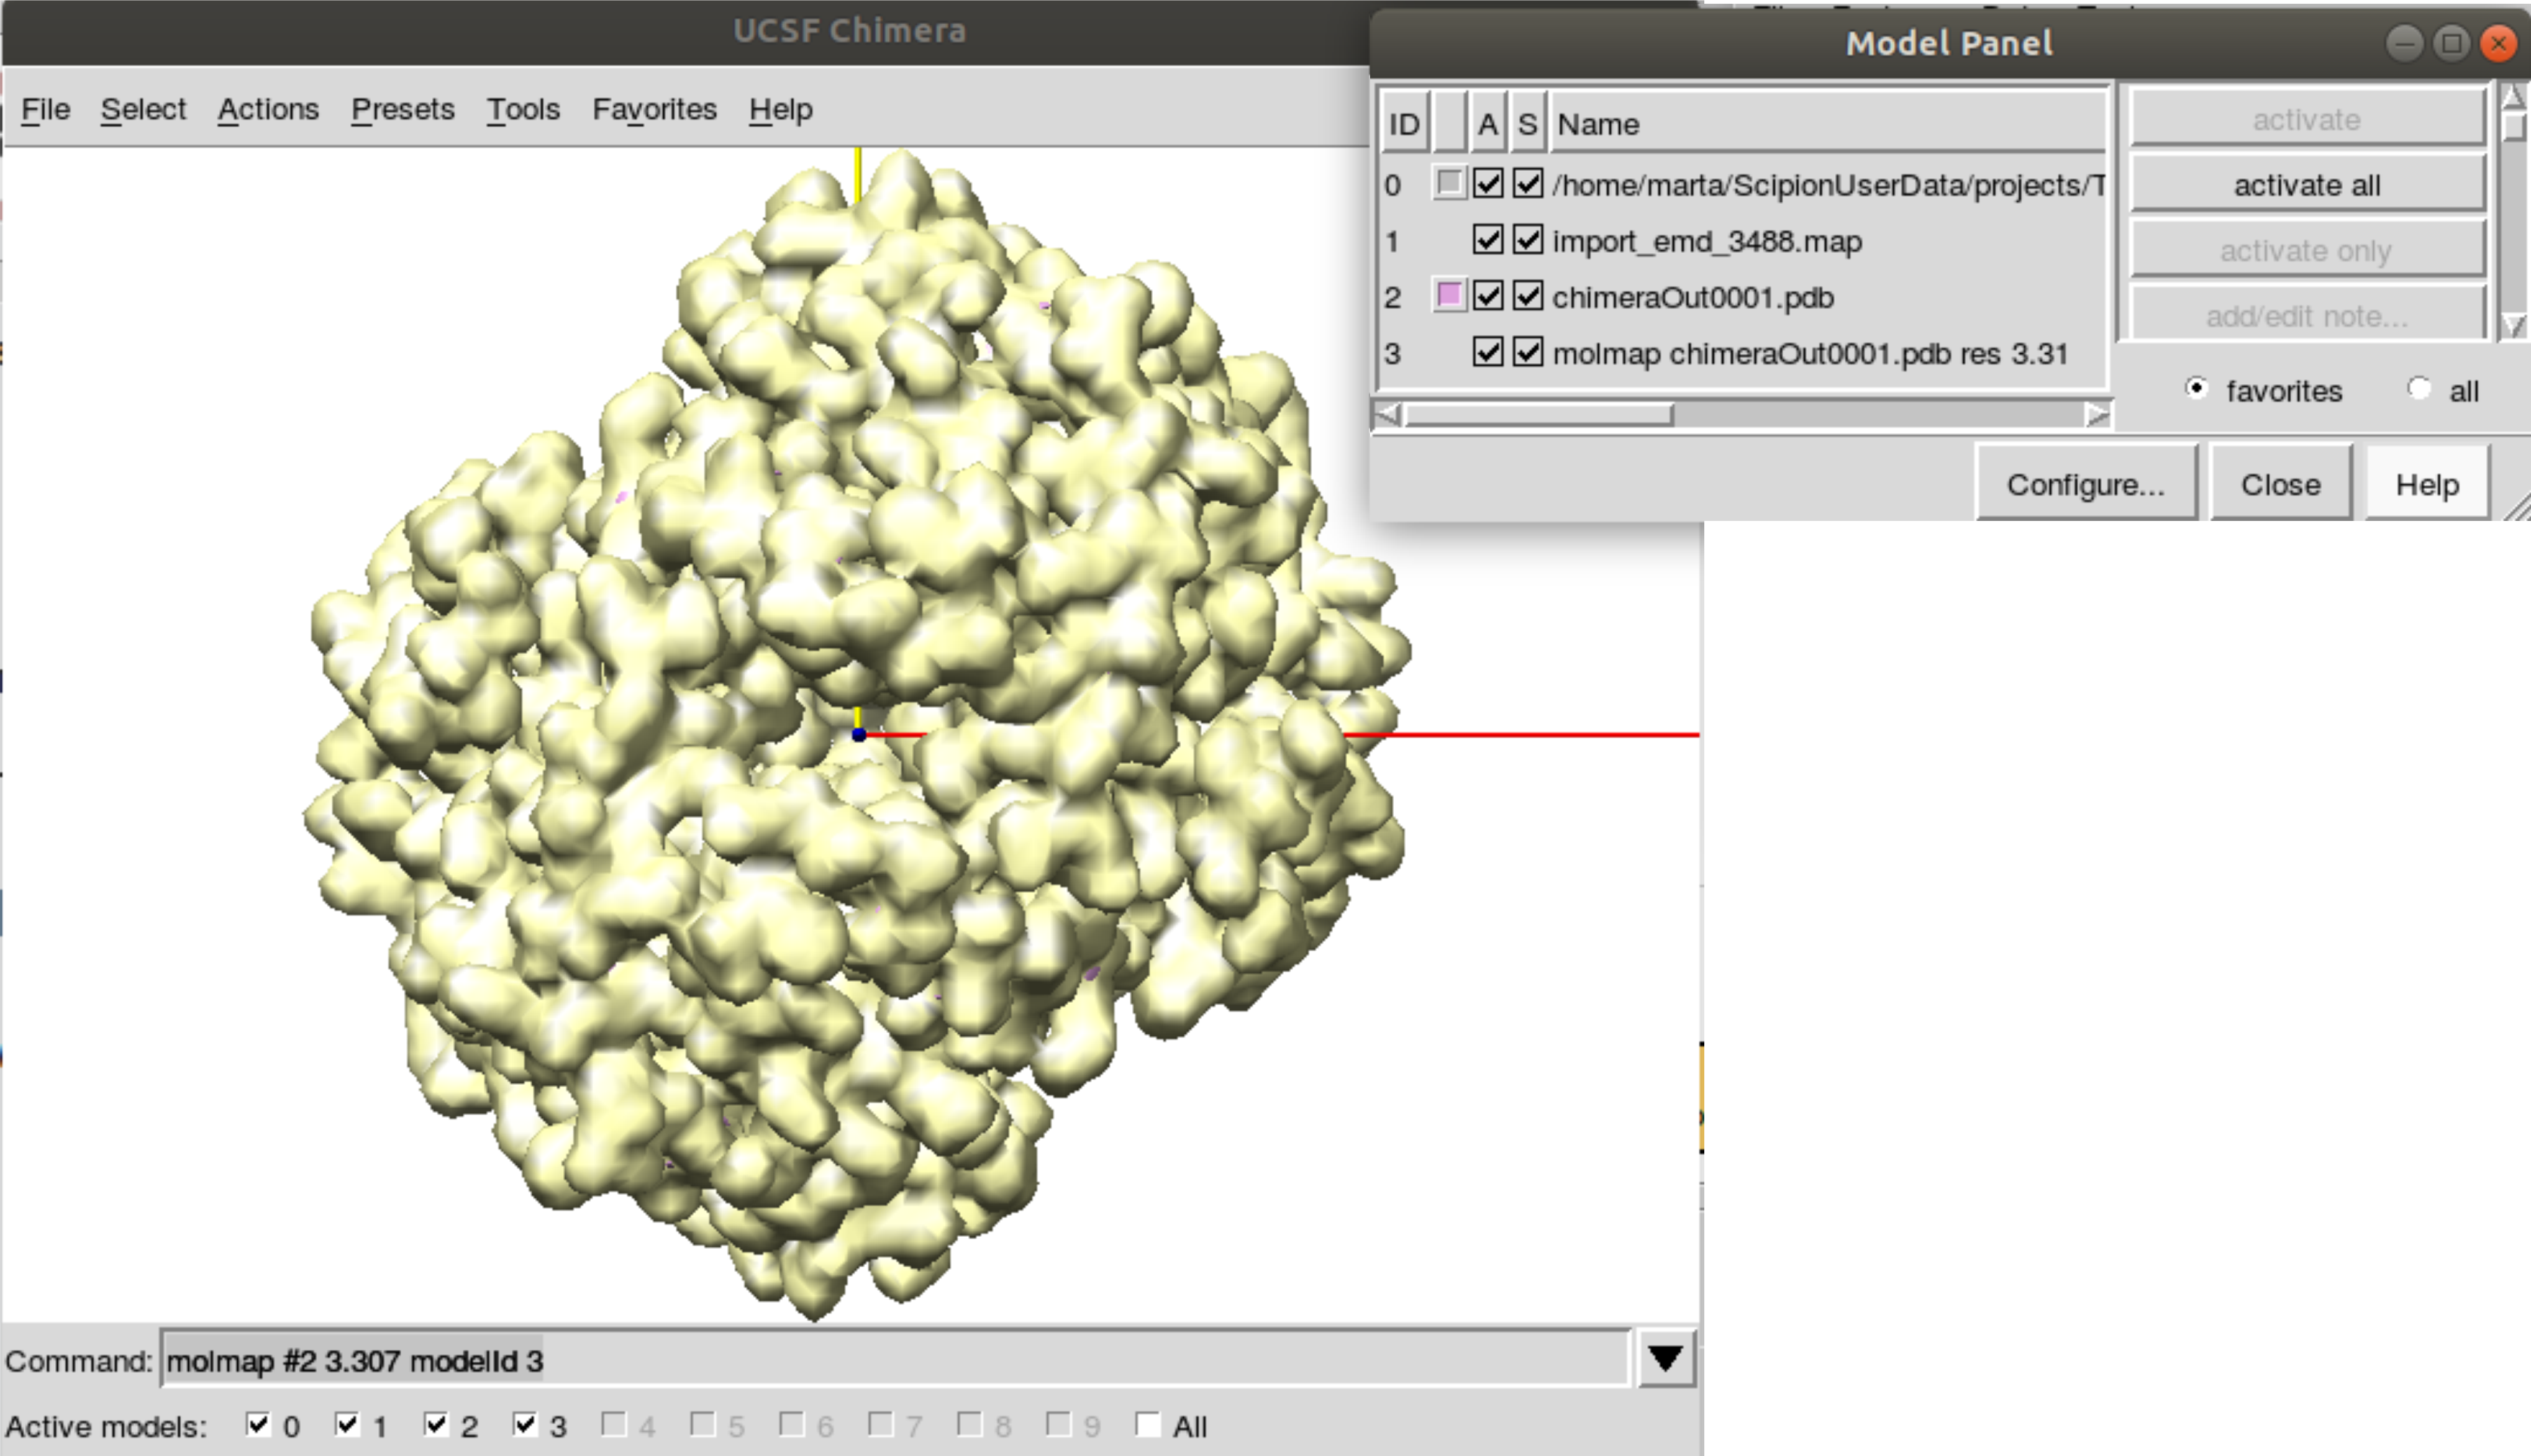
\includegraphics[width=0.90\textwidth]{Images/Fig43}
    \caption{Electron density volume generated from human \ttt{metHgb} $model$ in \chimera.}
    \label{fig:chimera_operate_vol_2}
   \end{figure}
  
  \item To subtract this new model from the starting whole volume \ttt{EMD-3488}, write in \chimera the command line:
  
  \begin{verbatim}
     vop subtract #1 #3 modelId #4 minRMS true
  \end{verbatim}
  where the minRMS option scales model \#3 automatically to minimize the root-mean-square sum of the resulting (subtracted) values at grid points within the lowest contour of model \#1.
  
  The resulting volume from this subtraction operation appears in \ffigure{fig:chimera_operate_vol_3} (\iii{Chimera model} \#4). From this result, we can conclude that most part of the initial density map has been traced, and there are no significant additional densities others than the four monomers and the four prosthetic groups that we have considered so far.
  
  \begin{figure}[H]
    \centering 
    \captionsetup{width=.7\linewidth} 
    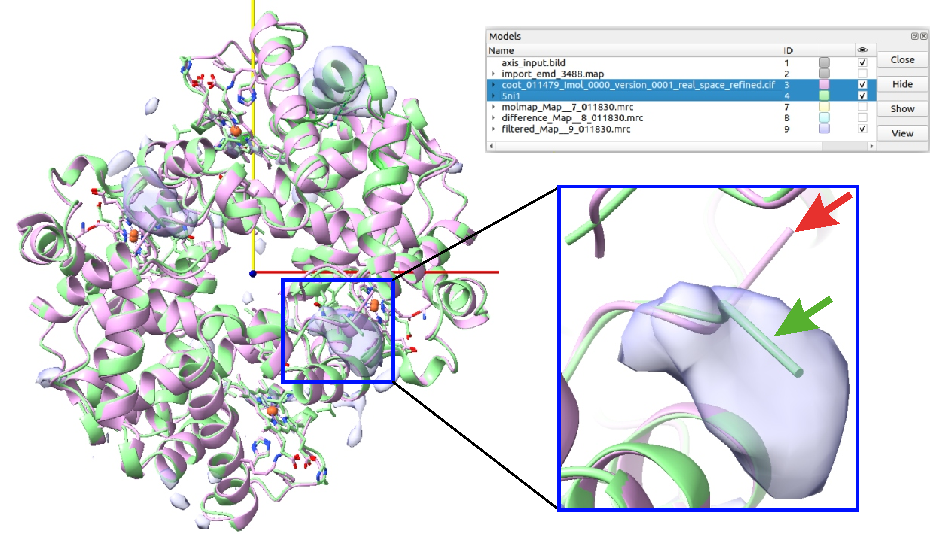
\includegraphics[width=0.90\textwidth]{Images/Fig44}
    \caption{Electron density difference between the starting volume \ttt{EMD-3488} and the volume generated from human \ttt{metHgb} $model$.}
    \label{fig:chimera_operate_vol_3}
   \end{figure}
  
  
  \end{itemize}
  
 % Traceback (most recent call last):
  %File "Atom_struct_out_8_009214.py", line 10, in <module>
   % aStruct1.addStruct(modelFileName[-1], '/home/marta/OLD/marta/ScipionUserData/projects/Demo_Modeling_2020/Runs/009214_ChimeraProtOperate/extra/%Atom_struct_out_8_009214.cif')
  %File "/home/marta/software/scipion3/scipion-em/pwem/convert/atom_struct.py", line 684, in addStruct
   % self._renameChainsIfNeed(struct2)
  %File "/home/marta/software/scipion3/scipion-em/pwem/convert/atom_struct.py", line 643, in _renameChainsIfNeed
   % chain.id = "%s%03d" % (cId[0], int(cId[1:]) + 1)
  %File "/home/marta/software/scipion3/scipion3env/lib/python3.6/site-packages/Bio/PDB/Entity.py", line 176, in id
   % "for a sibling of this entity.".format(self._id, value, value)
%ValueError: Cannot change id from `A002` to `A003`. The id `A003` is already used for a sibling of this entit
 
\end{itemize}
